\documentclass[a4paper,14pt]{extreport}
\usepackage[left=1.5cm,right=1.5cm,
    top=1.5cm,bottom=2cm,bindingoffset=0cm]{geometry}
\usepackage{scrextend}
\usepackage[T1,T2A]{fontenc}
\usepackage[utf8]{inputenc}
\usepackage[english,russian,ukrainian]{babel}
\usepackage{tabularx}
\usepackage{amssymb}
\linespread{1.5}
\usepackage{color}
\usepackage{amsmath}
\usepackage{mathrsfs}
\usepackage{listings}
\usepackage{graphicx}
\graphicspath{ {./images/} }
\usepackage{lipsum}
\usepackage{xcolor}
\usepackage{hyperref}
\usepackage{tcolorbox}
\usepackage{tikz}
\usepackage[framemethod=TikZ]{mdframed}
\usepackage{wrapfig,boxedminipage,lipsum}
\mdfdefinestyle{MyFrame}{%
linecolor=blue,outerlinewidth=2pt,roundcorner=20pt,innertopmargin=\baselineskip,innerbottommargin=\baselineskip,innerrightmargin=20pt,innerleftmargin=20pt,backgroundcolor=gray!50!white}
 \usepackage{csvsimple}
 \usepackage{supertabular}
\usepackage{pdflscape}
\usepackage{fancyvrb}
%\usepackage{comment}
\definecolor{ggreen}{rgb}{0.4,1,0}
\definecolor{rred}{rgb}{1,0.1,0.1}
\usepackage{array,tabularx}
\usepackage{colortbl}

\usepackage{varwidth}
\tcbuselibrary{skins}
\usepackage{fancybox}




\usepackage{float}
\usepackage{wrapfig}
\usepackage{framed}
%for nice Code{
\lstdefinestyle{customc}{
  belowcaptionskip=1\baselineskip,
  breaklines=true,
  frame=L,
  xleftmargin=\parindent,
  language=C,
  showstringspaces=false,
  basicstyle=\small\ttfamily,
  keywordstyle=\bfseries\color{green!40!black},
  commentstyle=\itshape\color{purple!40!black},
  identifierstyle=\color{blue},
  stringstyle=\color{orange},
}
\lstset{escapechar=@,style=customc}
%}


\begin{document}
\pagecolor{white}
\begin{titlepage}
  \begin{center}
    \large
    Національний технічний університет України \\ "Київський політехнічний інститут імені Ігоря Сікорського"


    Факультет Електроніки

    Кафедра мікроелектроніки
    \vfill

    \textsc{ЗВІТ}\\

    {\Large Про виконання лабораторної роботи №4\\
      з дисципліни: «Алгоритми та структури даних-2»\\[1cm]

      Використання списків для збереження та відображення графічної інформації.


    }

  \bigskip
\end{center}
\vfill

\newlength{\ML}
\settowidth{\ML}{«\underline{\hspace{0.4cm}}» \underline{\hspace{2cm}}}
\hfill
\begin{minipage}{1\textwidth}
Виконавець:\\
Студент 3-го курсу \hspace{4cm} $\underset{\text{(підпис)}}{\underline{\hspace{0.2\textwidth}}}$  \hspace{1cm}А.\,С.~Мнацаканов\\
\vspace{1cm}

Перевірив: \hspace{6.1cm} $\underset{\text{(підпис)}}{\underline{\hspace{0.2\textwidth}}}$  \hspace{1cm}Д.\,Д.~Татарчук\\

\end{minipage}

\vfill

\begin{center}
2021
\end{center}
\end{titlepage}
%--------------------------------1-------------------------------
%\begin{center}\fcolorbox{black}{ggreen}{Варіант № 5}\end{center}
\textbf{Мета роботи} – навчитись використовувати списки для тимчасового збереження великих об’ємів інформації..\\

\textbf{Завдання}\\
Написати програму, що виконує наступні дії:\\

1) Зчитує дані із файлу отриманого в першій лабораторній роботі та зберігає їх у пам’яті у вигляді структури заданої у таблиці 5 відповідно до варіанту завдань.\\

2) Визначає максимальний та мінімальний елементи списку.\\

3) Розраховує масштабні коефіцієнти для відображення графіку функції на екрані. Масштабні коефіцієнти повинні бути розраховані таким чином, щоб графік функції займав весь екран, як по вертикалі так і по горизонталі.\\

4) Відображати графік функції на екрані. Крім графіку на екрані повинні відображатись осі координат, масштабна сітка та значення по осях X та Y.\\



\vspace{0.3cm}
\begin{center}\textbf{Виконання роботи}\end{center}
\textbf{Код на С++}\\

\lstinputlisting[language=C++]{lab4.cpp}




\begin{figure}[h]
\center{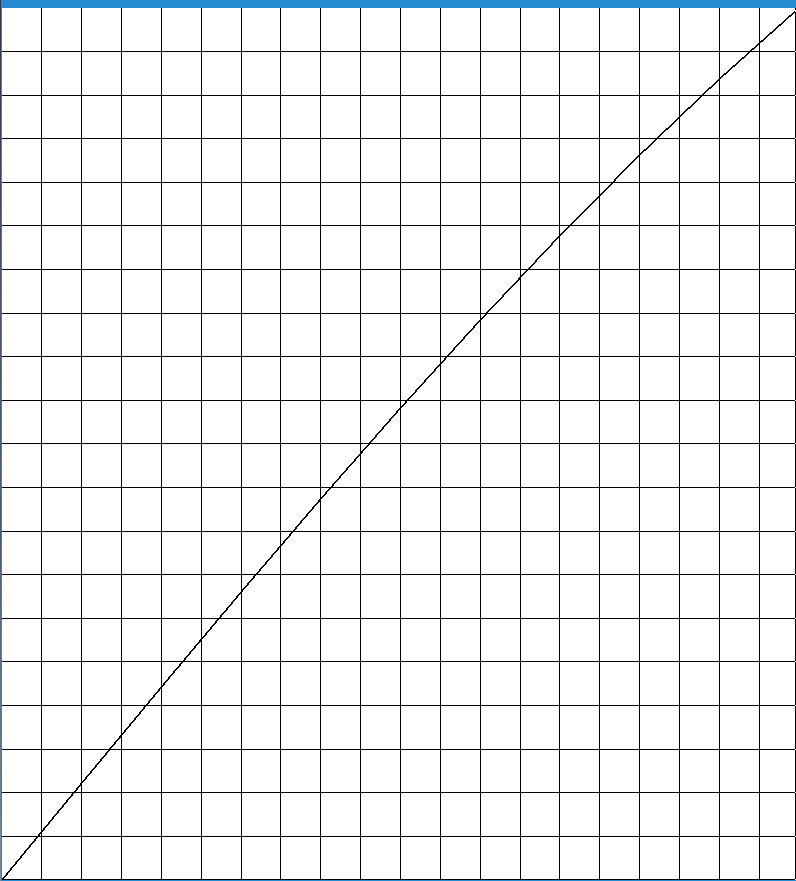
\includegraphics[width=0.6\linewidth]{1.png}}
\end{figure}

















\end{document}
